
% !TEX encoding = UTF-8 Unicode
% !program = pdflatex

\documentclass[11pt,a4paper,bibliography=totoc,listof=totocnumbered]{article}
\usepackage[a4paper,top=30mm,right=20mm,bottom=25mm,left=20mm,head=35mm,foot=15mm]{geometry}
\usepackage{fancyhdr}
\usepackage[parfill]{parskip}
\usepackage{algorithm}
\usepackage[noend]{algpseudocode}
\usepackage{amsmath}
\usepackage{mathtools}
\usepackage{listings}
\usepackage{color}
\usepackage[utf8]{inputenc} % Needed for the Umlaut in our title
\usepackage{pdfpages}
\usepackage{tikz}
\usetikzlibrary{decorations.pathreplacing}
\usepackage[style=numeric,sorting=none,backend=biber]{biblatex}
\addbibresource{citations.bib}

\definecolor{codegreen}{rgb}{0,0.6,0}
\definecolor{codegray}{rgb}{0.5,0.5,0.5}
\definecolor{codepurple}{rgb}{0.58,0,0.82}
\definecolor{backcolour}{rgb}{0.95,0.95,0.92}

\lstdefinestyle{mystyle}{
    backgroundcolor=\color{backcolour},   
    commentstyle=\color{codegreen},
    keywordstyle=\color{magenta},
    numberstyle=\tiny\color{codegray},
    stringstyle=\color{codepurple},
    basicstyle=\footnotesize,
    breakatwhitespace=false,         
    breaklines=true,                 
    captionpos=b,                    
    keepspaces=true,                 
    numbers=left,                    
    numbersep=5pt,                  
    showspaces=false,                
    showstringspaces=false,
    showtabs=false,                  
    tabsize=2
}
 
\lstset{style=mystyle}

% language
\usepackage[english]{babel}

% images
\usepackage[font=small,skip=6pt]{caption}
\usepackage{float,graphicx,grffile,wrapfig}
\graphicspath{ {images/} }

% variable definitions
\providecommand{\documenttitle}{Dynamic Event Detection in Data Streams}
\providecommand{\documentauthors}{
  David Pacassi Torrico,
  Daniel Milenkovic
}

\pagestyle{fancy}
\fancyhf{}
\lhead{\documenttitle}
\rhead{\nouppercase{\leftmark}}
\rfoot{Page \thepage}

\begin{document}

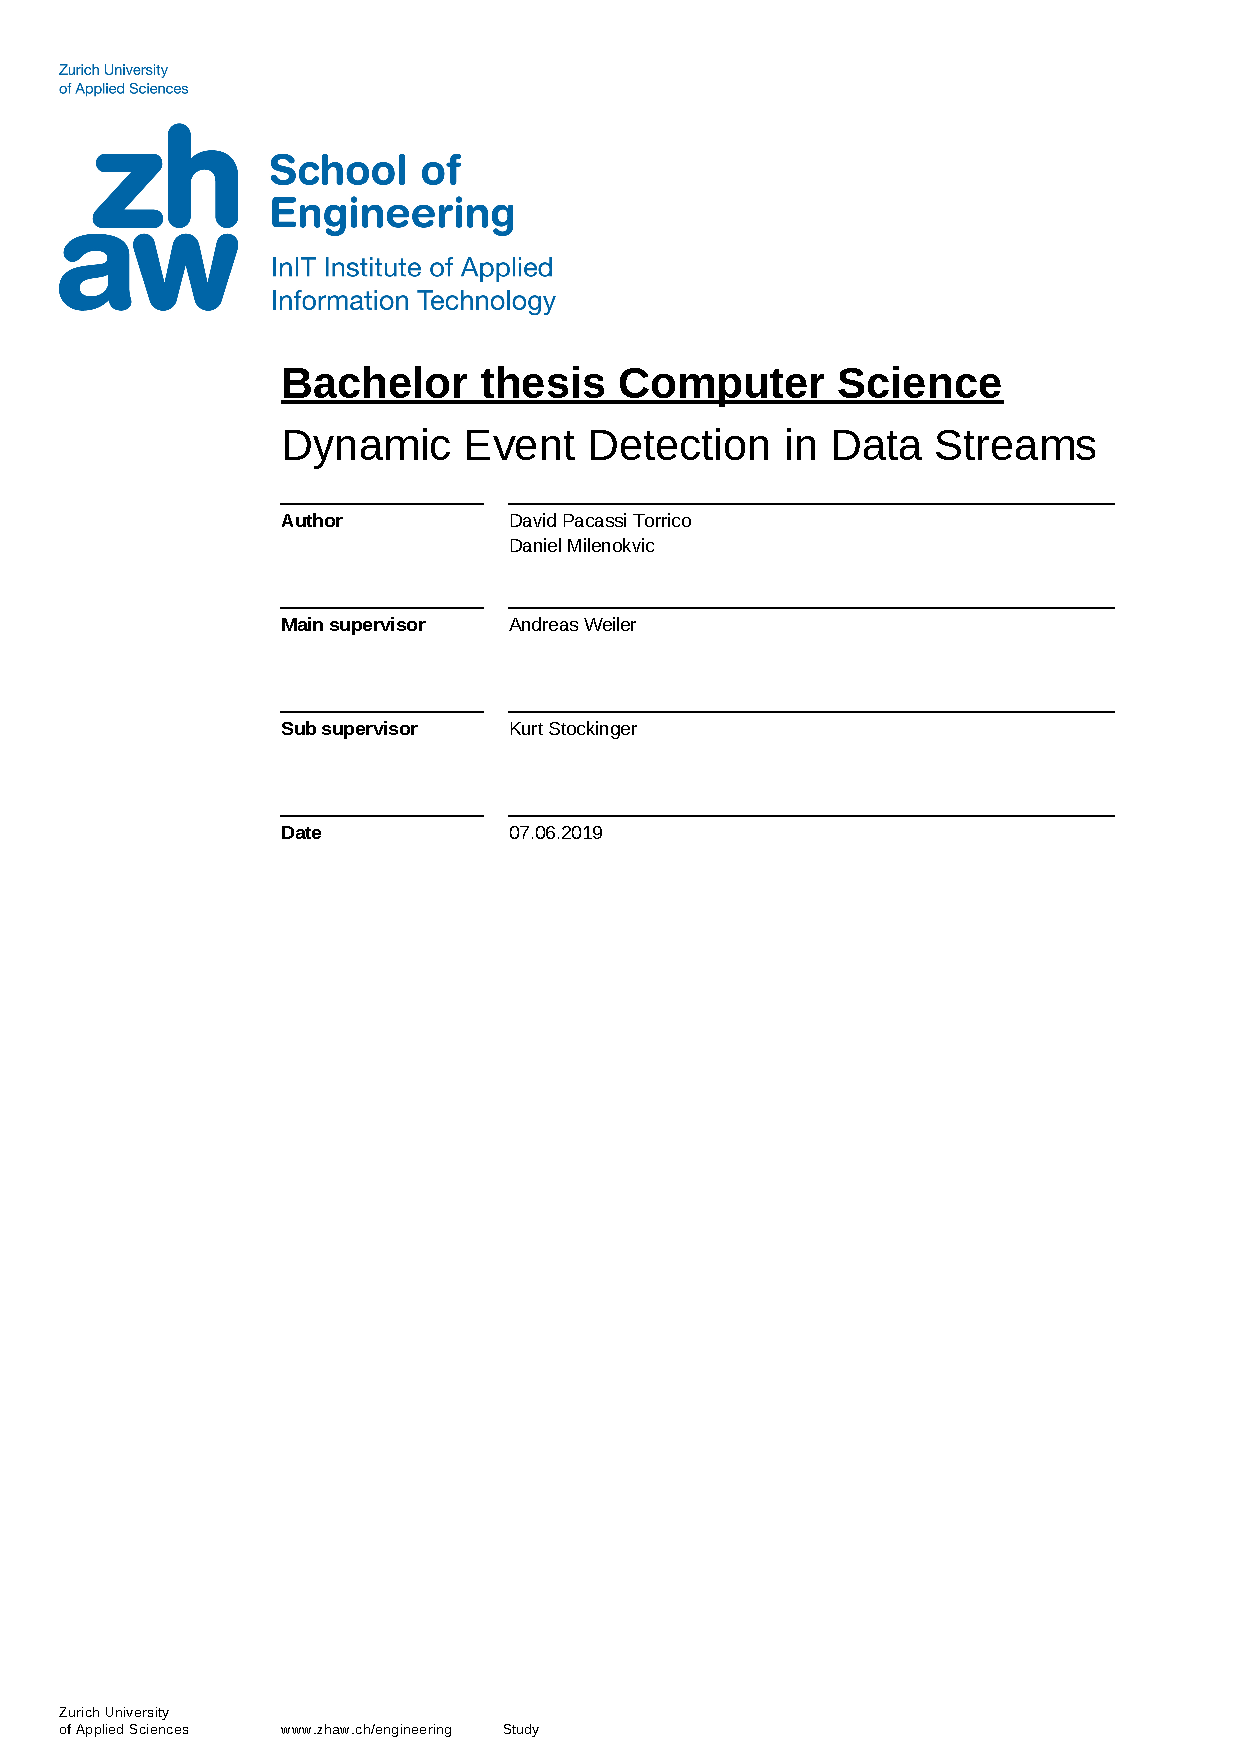
\includepdf{templates/cover.pdf}

\includepdf{templates/declaration_of_originality.pdf}

\section*{Abstract}
\label{sec:0_abstract}

Detecting events in data streams can be difficult,
especially if the definition, content, or properties of an event change over time.

This bachelor thesis focuses on the development and evaluation of an online clustering solution
in which events are defined either as changes in existing clusters or as the formation of new clusters.
The solution is a text mining software, which receives new news articles over a data stream and processes them.
Articles are assigned to different clusters due to their similarity to other articles.
The assumption is that very similar articles write about the same news story.
In addition, the evaluation of the clustering quality is measured with a custom scoring function.

The first part of this work consists of determining a suitable data set,
which will be the subject of the clustering and provides the ground truth for evaluating the results.
The implemented solution uses HDBSCAN as the clustering method
and compares it with the state-of-the-art method \textit{k}-means.
It turned out that the use of HDBSCAN has advantages over \textit{k}-means in terms of both performance and precision.
Furthermore, various text preprocessing methods and vector space models are evaluated,
with Text Lemmatization and tf-idf providing the most promising results.
Once applied in a simulated online setting,
the final evaluation found that the noise rate in the overall clustering reduces the precision in the event detection.

The resulting precision of the clustering is 72\% with a standard deviation of 12\%.
The precision for detecting new events results in 62\% with a standard deviation of 43\%.
Detecting changes in existing events results in a precision 69\% with a standard deviation of 16\%.
A continuation of this work should focus on improving the overall clustering to increase the precision of the event detection.

% Vorwort

\section{Preface}

The following bachelor thesis \textit{"Dynamic Event Detection in Data Streams"} was written
as part of our computer science studies at the ZHAW Zurich University of Applied Sciences.

After our lectures on artificial intelligence, we realized that we wanted to deepen our knowledge in this area.
This thesis was the perfect opportunity to increase our expertise on topics such as natural language processing
and cluster analysis.

Special thanks go to our two supervisors, Dr. Andreas Weiler and Prof. Dr. Kurt Stockinger,
for their ongoing and effective support during the writing of this thesis.

We would also like to thank our two lecturers Prof. Dr. Thilo Stadelmann
and Prof. Dr. Mark Cieliebak for their lectures on artificial intelligence.

At last but not least, we would like to thank our fellow students
and the entire ZHAW staff for our great time at ZHAW.

Daniel Milenkovic and David Pacassi Torrico

\tableofcontents\newpage

\section{Introduction}
\label{sec:introduction}

\subsection{Problem Formulation}
\label{sec:problem_formulation}
% Wie kann in einem Datenstrom Ereignisse erkannt werden?

% Bei der Suche nach neuen Ereignissen in Datenströmen, kommt es immer zum Problem was ein Ereignis genau ist. Wenn diese erste Frage geklärt ist kommt es aber zu weiteren Fragestellungen. Meistens reicht es nicht ein Ereignis statisch zu definieren, sondern die Definition entwickelt sich dynamisch über die Zeit. Die meisten Verfahren zu Ereigniserkennung werden aber bei Systemstart statisch eingestellt. Weiterhin muss man stets die Dynamik des Streams beachten, da es sonst du Blockaden und Überlauf im System kommen kann.

% Ziel dieser Arbeit ist es eine Methodik zu entwickeln wie die genannten Aspekte auf geeigneten Datenströmen umgesetzt werden können.


How can events be recognized in a data stream?
While searching for events in a data stream, the definition of an event is not always clear.
Providing static definitions, as most approaches do,
does not suffice for dynamic data streams, which change over time.
Additionally, the behaviour of the data stream is an important factor in itself,
since blockages of overflows in the system have to be prevented.

An example for a dynamic data stream can be found in a stream of news articles, which are published in irregular time intervals and different quantities over time. Thus detecting events based on an incoming stream of news articles is a challenging task.

The goal is to develop and evaluate a methodology to detect events in a dynamic stream of news articles.

\subsection{Motivation}
\label{sec:motivation}
Today's environment is rapidly changing.
With more devices being digitalized and connected to the internet,
we are starting to have incredible amounts of data.
Every smartphone, smartwatch and many other \gls{iot} devices start tracking every sensor data they record.

There is and will be no way to process all this data manually.
This is where our work becomes relevant.
We will try to detect events from a data stream, even when new and unknown events arise.

Our solution is based on text data, so any data in text form should be applicable.
With technologies such as speech recognition, the data could also initially be acoustic
and converted to text before being entered into our application.

That would open up use cases with smart speakers such as \textit{Amazon Echo} or \textit{Google Assistant}.

% lol stay humble david ;)
% \paragraph{Personal motivation}
% We have a combined experience of 17 years working in the IT sector together,
% for our bachelor thesis we wanted to do something more challenging than
% developing a simple application.

\section{Theoretical basics}

\subsection{Data Representation}

\subsubsection{Word Count}

\subsubsection{Tfidf}

\subsection{Clustering}
Clustering finds similarities in different news articles based on their content and groups them together, while unrelated news are regarded as noise. The challenge now araises to find an appropriate clustering method, which is able to work with data of varying densities and of high dimensionality.

TODO why hdbscan

\subsubsection{\textit{k}-means clustering}
\textit{k}-means clustering is an iterative clustering method which assigns all data points in a given data set
into k clusters, where k is a predefined number of clusters in the dataset.

% \subsubsubsection{How does k-means clustering work}
At the very beginning, k-means creates k centroids at random locations.
It then repeats following instructions until reaching convergence:

- For each data point: Find the nearest centroid
- Assign the data point to the nearest centroid (cluster)
- For each cluster: Compute a new cluster centroid with all assigned data points

% \subsubsubsection{Advantages}
- Very simple and easy to understand algorithm

% \subsubsubsection{Disadvantages}
- Initial (random) centroids have a strong impact on the results
- The number of clusters (k) has to be known beforehand
- Unable to handle noise (all data points will be assigned to a cluster)

\subsubsection{DBSCAN}
DBSCAN stands for *Density-Based Spatial Clustering of Applications with Noise*
and is a density based clustering algorithm.

A big advantage of DBSCAN is that it's able to sort data into clusters
of different shapes.

% \subsubsubsection{How does DBSCAN work}
DBSCAN requires two parameters in order to work:
1. epsilon - The maximum distance between two data points for them to be considered as in the same cluster.
2. minPoints - The number of data points a neighborhood has to contain in order to be considered as a cluster.

Having these two parameters defined, DBSCAN will iterate through the data points
and try to assign them to clusters if the provided parameters match.
If a data point can't be assigned to a cluster, it will be marked as noise point.

Data points that belong to a cluster but don't dense themselves are known
as **border points**. Some border points could theoretically belong to two or more clusters
if the distance from the point to the clusters don't differ.

% \subsubsubsection{Advantages}
- Does not need to know the number of clusters beforehand
- Is able to find shaped clusters
- Is able to handle noise points

% \subsubsubsection{Disadvantages}
- DBSCAN is not entirely deterministic
- Defining the right epsilon value can be difficult
- Unable to cluster data sets with large differences in densities

\subsubsection{HDBSCAN}

% Todo: check if we can re-use something of the commented draft.
\iffalse
HDBSCAN is a hierarchical density-based clustering algorithm \cite{McInnes2017}.
It extends the well known [insert citation] DBSCAN algorithm and reduces its sensitivity for clusters of varying densities.
Another important quality of HDBSCAN is, that it does not need to know the number of clusters up front.
\fi

HDBSCAN is a extension of DBSCAN that converts DBSCAN into a hierarchical clustering algorithm.
Therefor it only requires one parameter to be set:
1. minPoints - The number of data points a neighborhood has to contain in order to be considered as a cluster.

% \subsubsubsection{How does HDBSCAN work}
1. Transform the space according to the density/sparsity.
2. Build the minimum spanning tree of the distance weighted graph.
3. Construct a cluster hierarchy of connected components.
4. Condense the cluster hierarchy based on minimum cluster size.
5. Extract the stable clusters from the condensed tree.

% \subsubsubsubsection{1. Transforming the space}
One reason why HDBSCAN works so well, is that it is aware of noise.
This is very important as real life data is often messy and sometimes even corrupt.

Because of this, the very first thing HDBSCAN does, is to remove such data noise.
In order to identify noise, the **mutual reachability distance** score between
points is calculated. The mutual reachability distance score is defined as

TODO: Formula

whereas corek(x) stands for the core distance for a point x and a defined parameter k.

% \subsubsubsubsection{2. Building the minimum spanning tree}
TODO.


\section{Procedure}

TODO introductionary paragraph

\subsection{Data set}

The first important step is to create a test data set to run the evaluations with and verify them.

TODO explain the source and structrue

\subsubsection{Preprocessing}

% raw text
% with entity extraction
% word embeddings?
% Tfidf

\subsection{Experiments}

% Todo
Delete me
\subsection{Solution}

\subsection{Online Clustering}

Detecting events in a stream of news articles will be achieved by using an online clustering approach. The events of interest for this application are the discovery of new topics and the extension of existing topics. Thus we define our two events as follows:

\begin{itemize}
    \item Topic added: A new cluster of news articles appears in the data stream.
    \item Topic extended: An existing topic is extended by additional news articles.
\end{itemize}

HDBSCAN will be applied as the clustering method, using the optimal settings as discovered in the preivous evaluation. Additional preprocessing of news articles before clustering is going to be explored as part of evaluation as well and will be implemented accordingly for the online clustring.

Since HDBSCAN only supports static datasets, the clustering will be done in batches using a time based sliding window approach. Events are detected by comparing the resulting clusters with the previous ones.

\begin{figure}[h]
    \centering

    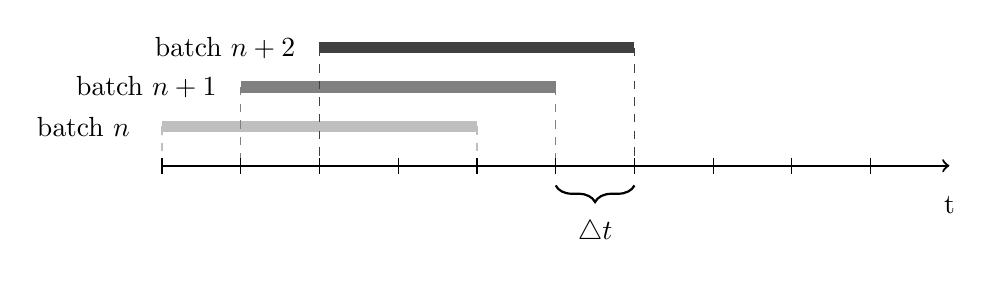
\begin{tikzpicture}[scale=1]


        \draw[lightgray, line width=4pt] (0,.5) -- (4,.5);
        \draw[lightgray, dashed] (0,.5) -- (0,0);
        \draw[lightgray, dashed] (4,.5) -- (4,0);
        \node[align=right] at (-1,.5) {batch $n$};

        \draw[gray, line width=4pt] (1,1) -- (5,1);
        \draw[gray, dashed] (1,1) -- (1,0);
        \draw[gray, dashed] (5,1) -- (5,0);
        \node[align=right] at (-.2,1) {batch $n + 1$};

        \draw[darkgray, line width=4pt] (2,1.5) -- (6,1.5);
        \draw[darkgray, dashed] (2,1.5) -- (2,0);
        \draw[darkgray, dashed] (6,1.5) -- (6,0);
        \node[align=right] at (0.8,1.5) {batch $n + 2$};

        \node[align=center] at (5.5,-0.85) {$\triangle t$};
        \node[align=center] at (10,-0.5) {t};

        \draw [thick,->] (0,0) -- (10,0);
        \foreach \x in {0,...,9} \draw (\x,0.1) -- (\x,-0.1);

        \draw [thick,decorate,decoration={brace,amplitude=6pt,raise=0pt,mirror}] (5,-0.25) -- (6,-0.25);

        \end{tikzpicture}

    \caption{Timeline showing the sliding window approach}
    \label{fig:timeline}
\end{figure}

\subsubsection{Finding pairs clusters}

To be able to compare clusters of different batches with each other, we have to find pairs of clusters between batches, which describe the same topic. This is done by applying the same assumptions as for the scoring function used in the evaluation. Therefore clusters are paired based on their similarity calculated with the jaccard index as shown in equation \ref{equ:similarity}. If the similarity is above a certain threshold, both clusters are seen as describing the same topic.

\subsubsection{Sliding window}

An important consideration for determining existing or new clusters is the overlap of samples between batches. If the overlap is too small, similar clusters will no longer be detected as such, which would result in an increasingly high error rate. Finding optimal values for the step size between batches and the number of samples for each batch is therefore essential for our online clustering approach.

\subsection{Model}

% Todo

delete me
\subsection{Software}

\subsubsection{Evaluation Framework}
The evaluation process is done with our own evaluation framework.
The framework allows for automated and repeatable evaluation runs.
Results are stored in a database for later analysis.
The main features include:

\begin{itemize}
    \item Defining the number of stories to run the evaluation with and load all news articles from those stories.
    \item Repeating evaluation runs with different sets of data.
    \item Providing different vectorizers for converting the textual data into a vector space model.
    \item Defining a range for each parameter of a clustering method and running it with each possible combination of those parameters.
    \item Storing the result the result in a database and creating relations between news articles, clusters and evaluation runs. This allows for manual inspection and analysis of individual articles inside a predicted cluster.
\end{itemize}

The implementation is done with Python. Clustering methods and vectorizers are provided by the Scikit-learn library. We decided to use Scikit-learn because of its rich documentation, the wide range of tools and algorithms it provides for clustering and our previous experience with it. Additionally the framework runs in a fully dockerized environment, which includes the database. This makes it very easy to run locally or on a server.

% TODO write it better

\subsubsection{Online Clustering}

* Near duplicate detection for clusters with MinHash and LSH O(log n)
* source https://towardsdatascience.com/understanding-locality-sensitive-hashing-49f6d1f6134

* simulate an dynamic stream from our static dataset

\subsection{Tests and validation}

\subsubsection{Scoring function}

The scoring function is essential for measuring the result of a clustering method. The score should reflect the quality of the individual clusters and of the clustering as a whole. The number of existing measures for clustering is vast and can be split into two main categories. Internal measures determine the score based on criteria derived from the data itself and external measures depend on criteria non-existent in the data itself such as class labels. Since the ground truth is known in our test data, we are going to apply an external measure.
Initially we used Normalized Mutual Information (NMI) as our primary scoring function. The NMI is a entropy-based measure and tries to quantify the amount shared information between the clusterings. The score proved to work well for our initial evaluations, but upon closer inspection certain anomalies were found. An example is given in table \ref{tab:nmi_kmeans_example}, where K-means achieved a rather high score, regardless of the significant difference between the true amount of clusters and the approximation using $\sqrt{n}$.

% TODO explain the reason for the big difference

TODO add number of estimated clusters
\begin{table}[h]
    \centering
    \begin{tabular}{|l|l|l|l|l|}
    \hline
    \textbf{Algorithm} & \textbf{Sample Size} & \textbf{NMI}  & $\mathbf{n_{true}}$ & $\mathbf{ \mid n_{true} - n_{predicted} \mid }$ \\ \hline
    k-means & 19255 & 0.754 & 600 & 457 \\ \hline
    hdbscan & 19255 & 0.742 & 600 & 2 \\ \hline
    \end{tabular}
    \caption{K-Means has a higher NMI score than HDBSCAN, while having a much larger difference in number of clusters.}
    \label{tab:nmi_kmeans_example}
\end{table}

Other scoring functions such as V-Measure or the Adjusted Rand Index showed similar unexpected results with different clusterings. Therefore we decided to develop our own scoring function based on the ideas of Maximum Matching and the jaccard index.

TODO find citations

\paragraph{Calculating the score}

The scoring function first calculates the similarity between pairs of clusters, where each cluster belongs to a different clustering. We use the jaccard index to measure the similarity, which is defined as

\begin{equation}
    \label{equ:similarity}
    \frac{|A \cap B|}{|A \cup B|}
\end{equation}

To illustrate the process we start with an example. We use $T$ and $C$ as our clusterings, where $T$ is the ground truth and $C$ is the predicted clustering. The clusterings are defined as follows:

\begin{gather*}
    T = \{\{1,2,3\},\{4,5,6,7\},\{8,9\}\} \\
    C = \{\{1,2\},\{3,4,5,6\},\{7\},\{8,9\}\}
\end{gather*}

We calculate the similarity as defined in Equation \ref{equ:similarity}, for each possible pair between $T$ and $C$ starting with $t_1= \{1,2,3\}$ and $c_1 = \{1,2\}$:

\begin{align*}
    similarity(t_1,c_1) &=\frac{|t_1 \cap c_1|}{|t_1 \cup c_1|}
    = \frac{|\{1,2\}|}{|\{1,2,3\}|}
    = \frac{2}{3} = 0.667 \\
\end{align*}

After doing this for each possible pair we get the similarity matrix $A$:

\begin{gather*}
\begin{array}{rcl}
    A = & \left(\begin{array}{cccc}
        similarity(t_1,c_1) & \hdots & \hdots & similarity(t_1,c_4)\\
        \vdots & \vdots & \vdots & \vdots\\
        similarity(t_3,c_3) & \hdots & \hdots & similarity(t_3,c_4) \end{array}\right)
        = & \left(\begin{array}{cccc}
            0.667 & 0.167 & 0 & 0 \\
            0 & 0.6 & 0.25 & 0.4 \\
            0 &  0 & 0 & 1.0 \end{array}\right)
\end{array}
\end{gather*}

As a next step we have to select the most relevant similarity values from each row of the similarity matrix.

Finding relevant values in the similarity matrix non-trivial, since clusters do not share labels across different clusterings. To solve this, we make two assumptions:
\begin{enumerate}
\item The higher the similarity between two clusters, the more likely it is, that both clusters are describing the same group of documents.
\item Each cluster can be associated with a cluster from another clustering only once.
\end{enumerate}

Based on those assumptions we select the highest similarity value per row, whose column is not already associated with another row. Applying this selection function $f$ to our previously calculated similarity matrix $A$ results in the set containing the most relevant similarity values.

\begin{gather*}
    \begin{array}{rcl}
        f(A) = & \left(\begin{array}{cccc}
            \mathbf{0.667} & 0.167 & 0 & 0 \\
            0 & \mathbf{0.6} & 0.25 & 0.4 \\
            0 &  0 & 0 & \mathbf{1.0} \end{array}\right)
            = \{0.667, 0.6, 1\}
    \end{array}
\end{gather*}

As we can see, there were no collisions between columns and we simply get the highest value per row. Consider the following example with an similarity matrix $B$, which does contain a collision:

\begin{gather*}
    \begin{array}{rcl}
        f(B) = & \left(\begin{array}{cccc}
            \mathbf{0.75} & 0.375 & 0.427 & 0.375 \\
            0.4 & \mathbf{0.667} & 0.571 & \textcolor{red}{0.8} \\
            0.333 &  0.25 & 0.4 & \mathbf{1.0} \end{array}\right)
            = \{0.75, 0.667, 1\}
    \end{array}
\end{gather*}

The selected similarity for the second row is 0.667 instead of 0.8. This is because the fourth column is already associated with the third row, while having an similarity greater than 0.8. Therefore based on our assumption that clusters cannot be associated twice, the second highest similarity is used for the second column. In case no association could be found, the value would be set to zero. The full algorithm for the selection process can be found in the appendix as listing \ref{lst:select_max_values}.

As a third step we have to calculate the weights to be used for the final  The weight is based on the number of elements inside the cluster and necessary to represent differences in predicted and true number of clusters in the final score. It is defined as follows

\begin{equation}
    \label{equ:weight}
        w_{ij} = \frac{|t_i| + |c_j|}{|T|+|C|} \\
\end{equation}

where $T$ is the ground truth with $t_i \in T$ and $C$ the predicted clustering with  $c_j \in C$. Therefore the weight for a pairing $t_ic_j$ includes both the size of the true cluster and the size of the predicted cluster. The reason both sizes are used, is that we want to reflect if the overall number of predicted clusters is different from the ground truth. Using only the true number of elements as the weight, would affect the score if |C| < |T|, but not |C| > |T|. Therefore the number of predicted elements has to be included as well.

In the fourth and final step we calculate the weighted average, $S$ is the similarity matrix with $s_{i} \in S$

\begin{equation}
    \label{equ:weighted_average}
        \text{MP-Score} = \sum_{i=0}^{|S|} w_is_i
\end{equation}

Where $S$ is the similarity matrix with $s_{i} \in S$ and $w_i$ the corresponding weight. Using our previously selected similarity values $S = f(A) = \{0.667, 0.6, 1\}$ with  $c_{true}=3$ and $c_{predicted}=4$, the calculation for the final average would be done as follows:

\begin{align*}
    score &= \frac{\sum_{i=1}^{|S|} S_i}{c_{true} + max(0, c_{predicted} - c_{true})} \\
    &= \frac{0.667 + 0.6 + 1}{3 + max(0, 4 - 3)} = \frac{2.267}{3 + max(0, 1)} \\
    &= \frac{2.267}{3 + 1} = \frac{2.267}{4} \\
    &= \mathbf{0.567}
\end{align*}

The final score for the evaluation of the predicted cluster $C$ with the true cluster is 0.567.

\paragraph{Comparison against other measures}

The test scenarios in table \ref{tab:score_scenarios} show the resulting scores of our similarity score, NMI and completeness. It is important to note that NMI and completeness work with cluster labels assigned to each document, instead of considing elements inside a single cluster. This means the clustering will be flattened into one dimension, where each document is assigned the label of the cluster it appeares in. The array containing the labels for the first scenario would look as follows: $C=[1,1,1,2,2,2,2,3,3]$.

\begin{table}[h]
    \centering
    \begin{tabular}{|l|l|l|l|l|}
    \hline
    \multicolumn{5}{ |c| }{\textbf{Test scenarios with ground truth $T = \{\{1,2,3\},\{4,5,6,7\},\{8,9\}\}$}} \\
    \hline
    Nr. & Predicted Clustering $C$ & NMI & ARI & MP-Score \\ \hline
    1 & $C = \{\{1,2,3\},\{4,5,6,7\},\{8,9\}\}$ & 1.0 & 1.0 & 1.0 \\ \hline
    2 & $C = \{\{1,2\},\{3,4,5,6\},\{7,8,9\}\}$ & 0.564 &  0.308 & 0.637 \\ \hline
    3 & $C = \{\{1,2,3\},\{4,5,6\},\{7\},\{8,9\}\}$ & 0.895 & 0.771 & 0.847 \\ \hline
    4 & $C = \{\{1,2,3\},\{4,5\},\{6,7\},\{8\},\{9\}\}$ & 0.821 & 0.591 & 0.583 \\ \hline
    5 & $C = \{\{1\},\{2\},\{3\},\{4\},\{5\},\{6\},\{7\},\{8\},\{9\}\}$ & 0.651 & 0 & 0.227 \\ \hline
    6 & $C = \{\{1,2,3,4,5\},\{6,7,8,9\}\}$ & 0.434 & 0.182 & 0.433 \\ \hline
    7 & $C = \{\{1,2,3,4,5,6,7,8,9\}\}$ & 0.0 & 0 & 0.321 \\ \hline
    8 & $C = \{\{7,2,4\},\{8,9,6,3\},\{1,5\}\}$ & 0.219 & -0.108 & 0.392 \\ \hline
    \end{tabular}
    \caption{Direct comparison of different scoring functions}
    \label{tab:score_scenarios}
\end{table}

As a final note, repeating the evaluation shown in table \ref{tab:nmi_kmeans_example} a second time using the MP-Score, the score (Table \ref{tab:avg_predict_kmeans_example}) for K-means is much lower than HDBSCAN. This reflects what we would expect based on the big difference in the amount of predicted clusters.

\begin{table}[h]
    \centering
    \begin{tabular}{|l|l|l|l|l|}
    \hline
    \textbf{Algorithm} & \textbf{Sample Size} & \textbf{Similarity}  & $\mathbf{n_{true}}$ & $\mathbf{ \mid n_{true} - n_{predicted} \mid }$ \\ \hline
    k-means & 19255 & 0.137 & 600 & 457 \\ \hline
    hdbscan & 19255 & 0.605 & 600 & 2 \\ \hline
    \end{tabular}
    \caption{The similarty score reflects the difference in number of predicted clusters.}
    \label{tab:avg_predict_kmeans_example}
\end{table}

\section{Results}

\subsection{Clustering method}

The goal of this evaluation is to measure the accuracy of HDBSCAN, with different parameters and preprocessing methods. The most suitable approach will then be used for the online clustering to detect changes in a news stream.

\subsubsection{Setup}

\paragraph{Text Preprocessing}

 The first step in working with text is to apply Natural Language Processing techniques for improving the quality of the data before clustering it. We look the five different preprocessing methods  as described in section \ref{} and evaluate each. The methods are:
 \begin{itemize}
     \item Full text with stop word removal
     \item Keyterms
     \item Named Entities
     \item Lemmatization
     \item Stemmatization
 \end{itemize} 

\paragraph{Text Vectorization} Before the text can be clustered, it has to be transformed into a vector space model. We look at two different models:
\begin{itemize}
    \item Word Count
    \item Tfidf
\end{itemize}

\paragraph{Parameters} HDBSCAN has a range of parameters, which can be tuned to fit our dataset. We focus on the two primary ones:
\begin{itemize}
    \item Min cluster size: The minimum size of a cluster. We run the evaluation with a range from two to nine as the $min\_cluster\_size$. 
    \item Metric: The distance measure between points. We apply the metrics "cosine" and "euclidean". 
    
\end{itemize}

The primary parameter for K-Means is the number of clusters. Since K-Means is used as a baseline to evaluate HDBSCAN, we provide the true number of clusters for each run. Therefore K-Means runs with an optimal starting point. 

\paragraph{Running the evaluation} The evaluation is done with different sets of news articles per run. This means if we define a run to use 30 stories and set it to repeat five times, each repeat will load 30 different stories from the dataset. This is done to get a more diverse set of samples. Each run will be repeated at least three times. Lower numbers of stories allow for more repetitions due to lower processing times.   

\subsubsection{Evaluation}

The first run is done with 60 stories, which results in approximately 2000 news articles, over five repetitions. Table \ref{tab:cluster_parameters} shows the resulting accuracy for each parameter in combination with each preprocessing method and vector space model. The highest score per parameter is highlighted as bold. The first insight we get is the variety in accuracy scores for different min cluster sizes. The lowest min cluster size results in the lowest accuracy, while increasing this parameter leads to an increasingly better score. The highest accuracy is reached with a min cluster size of six, while increasing it further reduces the score again. The large difference in accuracies between different min cluster sizes, shows the importance this parameters has on the quality of the clustering and requires some knowledge of the data beforehand. In our case we have a wide range of different cluster sizes as shown in figure \ref{fig:articles_per_story_distribution}, with clusters containing as little as two news articles. Based on this distribution we expected the min size cluster size to be low. The distribution also explains the drop in accuracy after a min cluster size of 6, since an increasingly number of clusters are being ignored.

\begin{table}[h]
    \centering
    \scalebox{0.65}{
    \begin{tabular}{|l|rrrrr|rrrrr|}
        \hline
        \textbf{Clustering} & \multicolumn{5}{ |c| }{\textbf{Word Count}} & \multicolumn{5}{ |c| }{\textbf{Tfidf}} \\
        \hline
        \textbf{HDBSCAN} & Full Text &  Keyterms & Entities & Lemmatized & Stemmed & Full Text &  Keyterms & Entities & Lemmatized & Stemmed \\
        \hline
        min\_size: 2, metric: cosine    & 0.289 & 0.265 & 0.223 & \textbf{0.305} & 0.297 & 0.286     & 0.268 & 0.26      & 0.296     & 0.3       \\
        min\_size: 2, metric: euclidean & 0.101 & 0.093 & 0.110 & 0.101     & 0.106 & 0.301     & 0.170 & 0.241     & \textbf{0.306} & 0.301     \\
        min\_size: 3, metric: cosine    & 0.488 & 0.456 & 0.465 & 0.48      & 0.487 & 0.472     & 0.446 & 0.457     & \textbf{0.493} & 0.478     \\
        min\_size: 3, metric: euclidean & 0.172 & 0.129 & 0.176 & 0.174     & 0.182 & 0.472     & 0.306 & 0.464     & \textbf{0.500} & 0.478     \\
        min\_size: 4, metric: cosine    & 0.630 & 0.555 & 0.625 & 0.552     & 0.577 & 0.577     & 0.586 & \textbf{0.646} & 0.589     & 0.581     \\
        min\_size: 4, metric: euclidean & 0.320 & 0.182 & 0.214 & 0.315     & 0.332 & 0.611     & 0.416 & 0.559     & 0.613     & \textbf{0.615} \\
        min\_size: 5, metric: cosine    & 0.716 & 0.652 & 0.656 & \textbf{0.718} & 0.718 & 0.688     & 0.664 & 0.632     & 0.686     & 0.692     \\
        min\_size: 5, metric: euclidean & 0.355 & 0.217 & 0.266 & 0.41      & 0.389 & \textbf{0.703} & 0.512 & 0.607     & 0.686     & 0.692     \\
        min\_size: 6, metric: cosine    & 0.693 & 0.715 & 0.608 & 0.701     & 0.708 & 0.738     & 0.729 & 0.613     & \textbf{0.751} & 0.747     \\
        min\_size: 6, metric: euclidean & 0.179 & 0.280 & 0.292 & 0.202     & 0.164 & 0.738     & 0.408 & 0.622     & \textbf{0.778} & 0.763     \\
        min\_size: 7, metric: cosine    & 0.631 & 0.611 & 0.552 & 0.643     & 0.634 & 0.689     & 0.685 & 0.553     & 0.718     & \textbf{0.722} \\
        min\_size: 7, metric: euclidean & 0.122 & 0.392 & 0.307 & 0.073     & 0.099 & 0.689     & 0.336 & 0.539     & 0.718     & \textbf{0.722} \\
        min\_size: 8, metric: cosine    & 0.571 & 0.603 & 0.514 & 0.592     & 0.574 & 0.685     & 0.647 & 0.531     & \textbf{0.711} & 0.695     \\
        min\_size: 8, metric: euclidean & 0.056 & 0.339 & 0.338 & 0.025     & 0.057 & 0.685     & 0.286 & 0.522     & \textbf{0.711} & 0.695     \\
        min\_size: 9, metric: cosine    & 0.542 & 0.569 & 0.476 & 0.544     & 0.541 & 0.602     & 0.614 & 0.499     & 0.637     & \textbf{0.640} \\
        min\_size: 9, metric: euclidean & 0.065 & 0.236 & 0.310 & 0.025     & 0.033 & 0.602     & 0.216 & 0.475     & 0.637     & \textbf{0.640} \\
        \hline
        \textbf{K-Means} & \multicolumn{5}{ |c| }{}  & \multicolumn{5}{ |c| }{} \\
        \hline
        n\_cluster: n\_true              & 0.531 & 0.588 & 0.514 & 0.536     & 0.536 & \textbf{0.713} & 0.653 & 0.584     & 0.672     & 0.693     \\
        \hline
    
    \end{tabular}   
    }
    \caption{Accuracy for combinations of parameter and preprocessing with a sample size of 60 stories (approx. 2000 articles)}
    \label{tab:cluster_parameters}
\end{table}

Comparing the two vector models, shows the majority of best scores per parameter achieved by Tfidf. Additionally the different metrics show a significant difference when using the vector model based on word count. With Tfidf the difference between both metrics is often negligible.

As for the optimal preprocessing, lemmatization appears to provide the highest accuray in general or at least being fairly close to the highest score. This is to be expected, since lemmatization reduces the dimensions by grouping words into their base form, while still retaining most of the text. In contrast to keyterm and entity extraction, which both result in a drastic reduction of the dimensions, and therefore less detail. It is important to note, that we used pretrained models for keyterm and entity extraction. Specifically training on a news corpus might improve the performance of both methods, but it was decided as to be out of scope for this thesis.

\begin{figure}[h]
    \centering
    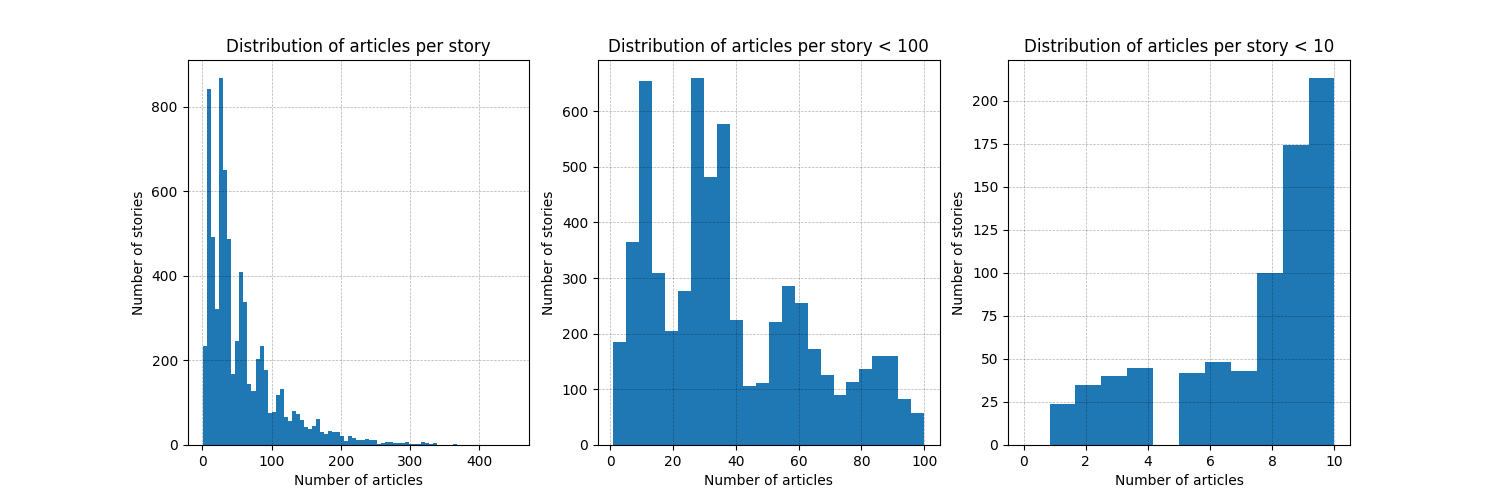
\includegraphics[width=1\textwidth]{articles_per_story_distribution}
    \caption{Distribution of cluster sizes.}
    \label{fig:articles_per_story_distribution}
\end{figure}

After determining the optimal settings for text preprocessing and vectorization, we increase the sample sizes for our evaluation runs, to get a deeper insight into the behaviour of HDBSCAN with larger datasets. Figure \ref{fig:hdbscan_parameters} shows the scores achieved with different parameters over an increasingly large set of samples. Based on this figure we see the metric $cosine$ to be generally better than $euclidean$, even if $euclidean$ is occasionally more accurate.

TODO explain why cosine is generally better than euclidean
TODO explain min cluster sizes, but run with lemmatization

\begin{figure}[h]
    \centering
    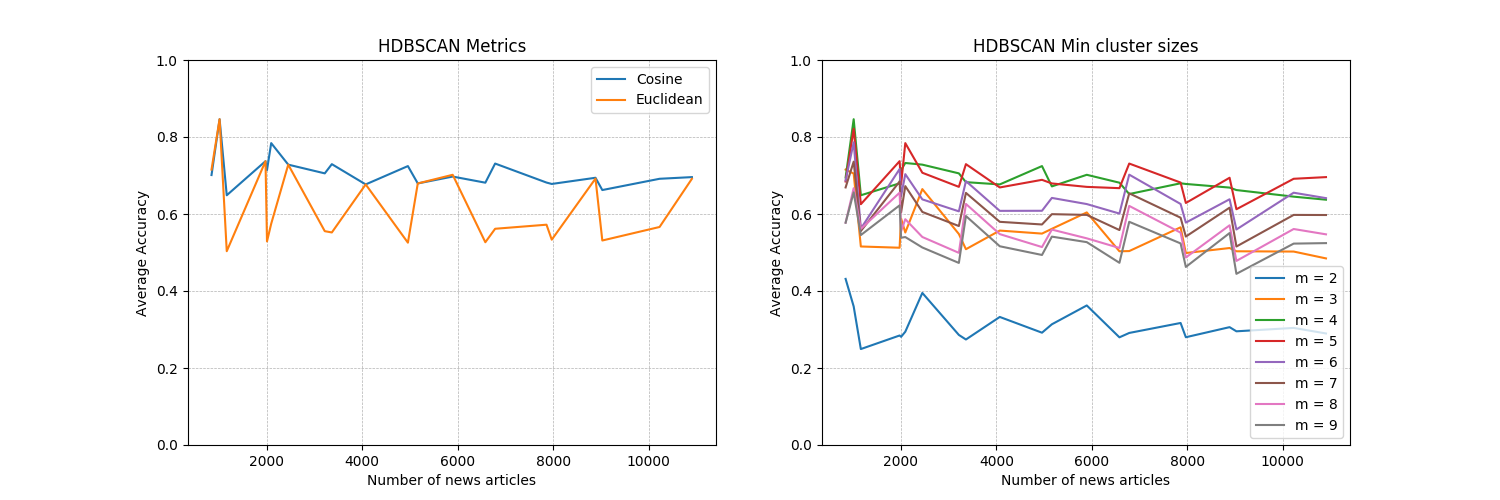
\includegraphics[width=1\textwidth]{hdbscan_parameters}
    \caption{Accuracies for different parameters}
    \label{fig:hdbscan_parameters}
\end{figure}

One of the advantages HDBSCAN has over other clustering algorithms, is the ability to work with noise, since we intent on applying it in an online setting, where noisy data is to be expected. At the same time, the number of articles classified as noise should be kept to a minimum. However the noise ratio shown in Figure \ref{fig:noise_ratio_samples} is higher, than we would expect it to be based on our test data. A variety of factors play into the high noise ratio. One major influence is due to the used $min\_cluster\_size$. Each news article belonging to a cluster ignored due to a size too small, will be counted as noise. In addition to the false positives due to the min cluster size, the test data does still contain noisy data, even after our efforts in cleaning up the data as good as possible. Nontheless the expected noise ratio based on the test data is less than 10\%, nowhere close to the 20\% of the current evaluation. Decreasing the noise ratio is certainly an important part in future improvements.

TODO calculate expected noise ratio based our min cluster sizes.

% experiment with min_samples

\begin{figure}[h]
    \centering
    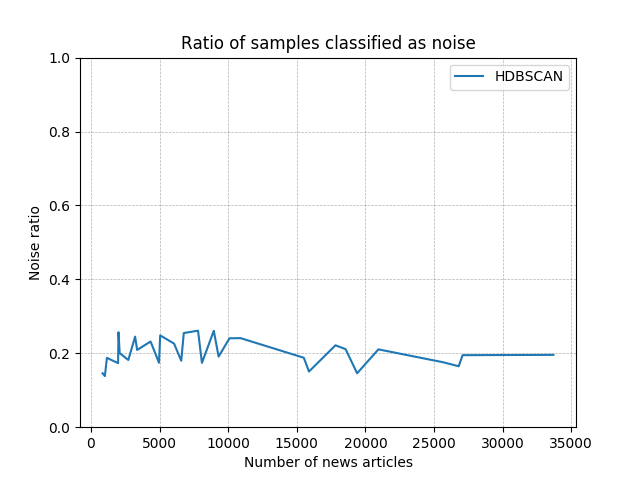
\includegraphics[width=0.5\textwidth]{noise_ratio_samples}
    \caption{Number of news articles classified as noise.}
    \label{fig:noise_ratio_samples}
\end{figure}


Having found the optimal settings to run HDBSCAN with, we can start comparing the overall performance with K-Means. Figure \ref{fig:accuracy_kmeans_hdbscan} shows  a similar behaviour for both clustering methods in value and variance of the accuracy. Although HDBSCAN is generally more accurate than K-Means, the difference gets smaller with an increase in the sample size. 

Increasing the sample size results for both HDBSCAN and K-means in a small loss regarding the accuracy as can be seen in figure \ref{fig:accuracy_kmeans_hdbscan}. However the accuracy seems to stabilize around the 0.7 mark.

\begin{figure}[h]
    \centering
    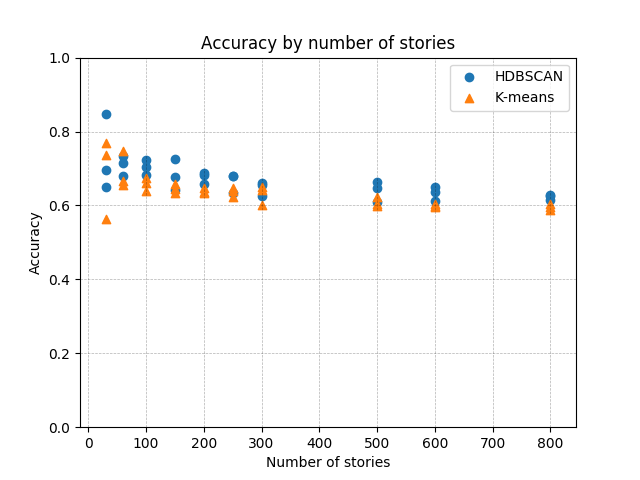
\includegraphics[width=0.5\textwidth]{accuracy_kmeans_hdbscan}
    \caption{Comparison of the average accuracy between K-means and HDBSCAN}
    \label{fig:accuracy_kmeans_hdbscan}
\end{figure}

While HDBSCAN and K-means provide a similar accuracy, the biggest difference can be noted in the processing time in relation to the number of samples. K-means has a time complexity of $O(n^2)$ in contrast to HDBSCAN with a time complexity of $O(nlog(n))$, which is demonstrated by figure \ref{fig:processing_time_kmeans_hdbscan}. Although running the evaluation has also shown the space complexity for HDBSCAN to be substantially higher for larger amounts of samples than with K-means. Trying to run HDBSCAN with 100'000 news articles caused in a memory error, even with 64GB of RAM, while K-means was able to complete the clustering.

% TODO measure memory?

\begin{figure}[h]
    \centering
    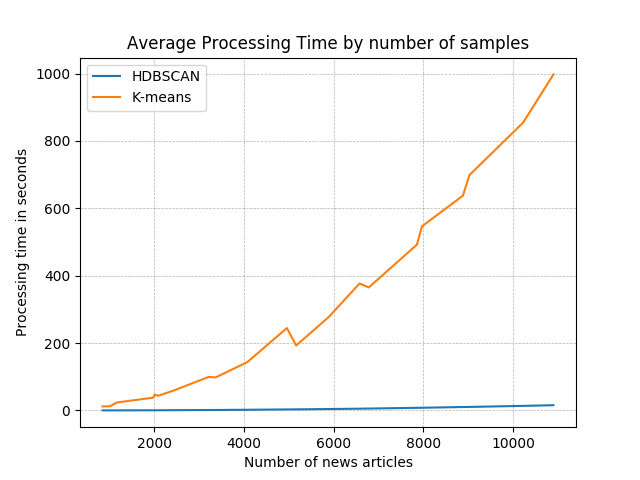
\includegraphics[width=0.5\textwidth]{processing_time_kmeans_hdbscan}
    \caption{Processing time in seconds }
    \label{fig:processing_time_kmeans_hdbscan}
\end{figure}

Figure \ref{fig:cluster_difference_samples} shows, that the difference between predicted over the true number of clusters is fairly low and appears to be roughly linear with the overall number of clusters.  

\begin{figure}[h]
    \centering
    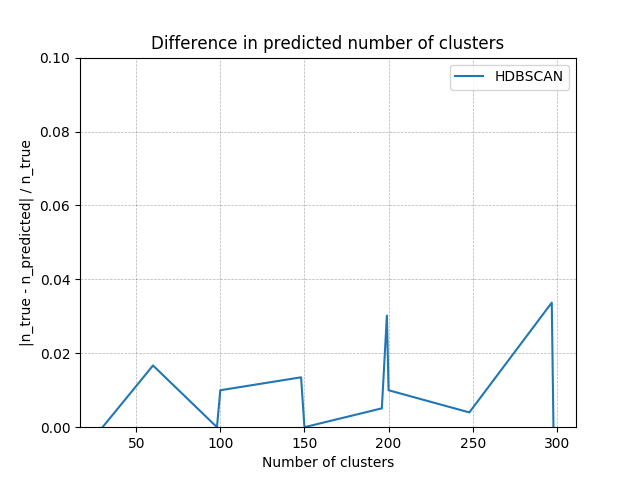
\includegraphics[width=0.5\textwidth]{cluster_difference_samples}
    \caption{Ratio of difference over predicted with true number of clusters}
    \label{fig:cluster_difference_samples}
\end{figure}

As a final note, we compare HDBSCAN with six different clustering methods taken from scikit-learn. Each method is run with a variety of parameters and the best scores are shown in figure \ref{fig:different_clusterings}. HDBSCAN provides the highest accuracy, while being still being one of the fastest algorithms. Based on this data, we can assume HDBSCAN to be a good candidate for our use case.

\begin{figure}[h]
    \centering
    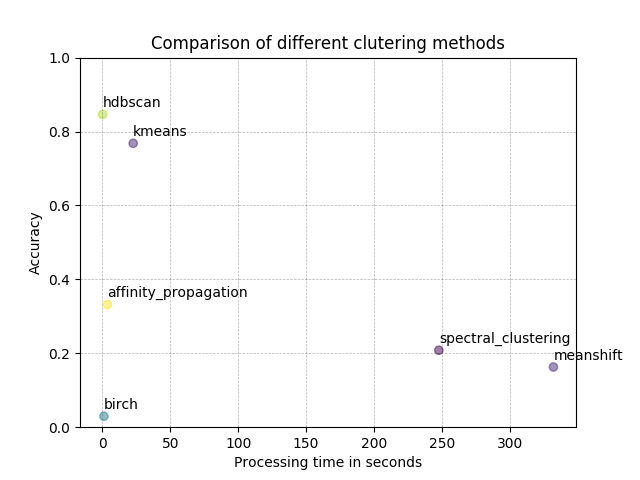
\includegraphics[width=0.5\textwidth]{different_clusterings}
    \caption{Comparison of different clustering methods with a sample size of approximately 1000 news articles}
    \label{fig:different_clusterings}
\end{figure}

\subsubsection{Conclusion}

The evaluation has shown HDBSCAN to be a good candidate to use for news clustering. It provides an better accuracy than K-means, while being significantly faster to process. The predicted number of clusters is consistent with an increasing number of samples and fairly close the truth. Additionally we have shown the required preprocessing and vectorization steps with the ideal parameters to achieve the most accurate results for our dataset. On the flip side the noise ratio is quite high and the space complexity is problematic with larger datasets. Overall HDBSCAN provides an acceptable accuracy, while still leaving room for further improvements.

\subsection{Evaluation of online clustering}

TODO new topic, topic extended

TODO cluster stability

\begin{figure}[h]
    \centering
    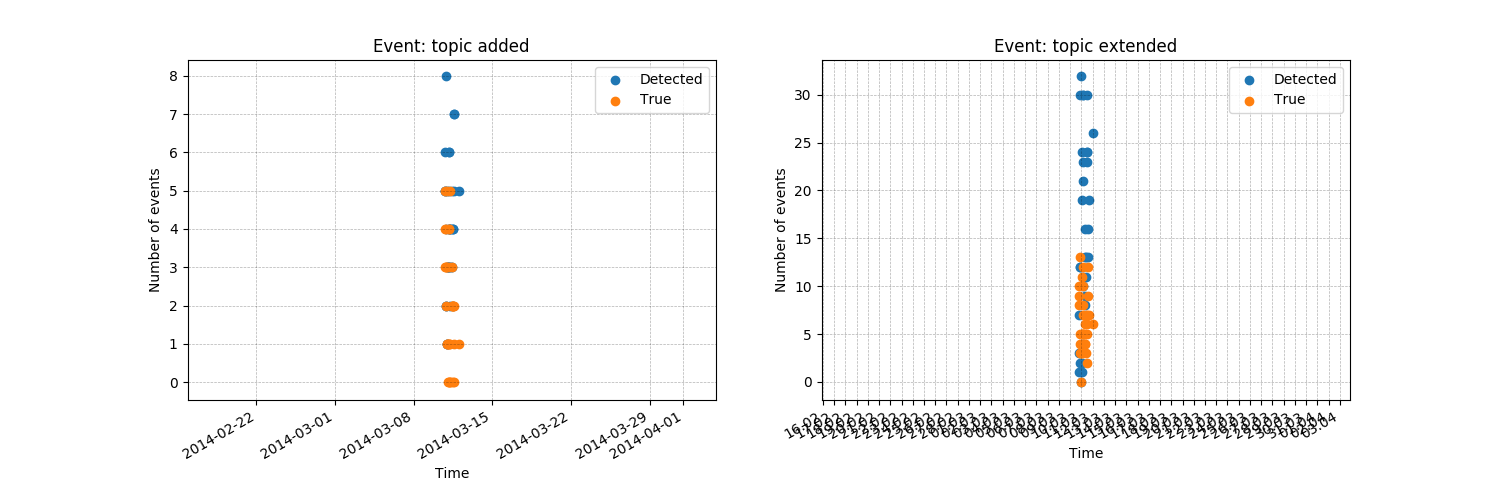
\includegraphics[width=1\textwidth]{event_detection_by_date}
    \caption{Comparison between detected and true events}
    \label{fig:event_detection_by_date}
\end{figure}

\begin{figure}[h]
    \centering
    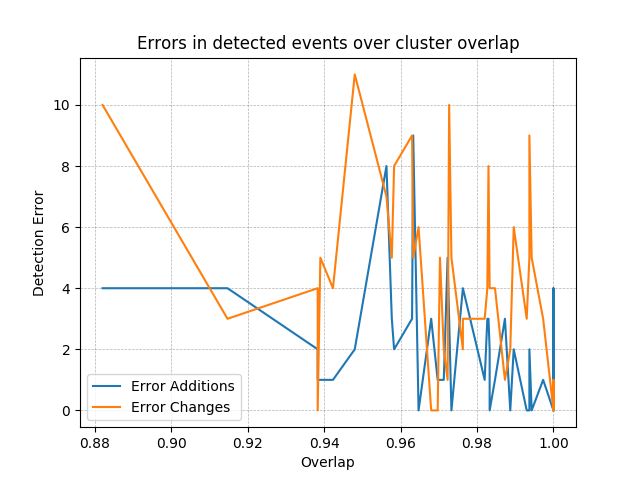
\includegraphics[width=0.5\textwidth]{event_detection_overlap}
    \caption{Plot work in progress}
    \label{fig:event_detection_overlap}
\end{figure}

% analyse overlap size
% show incoming news articles
% show deletion events on full clusterings
\section{Conclusion}

\subsection{Summary}

Short summary of this work.

\subsection{Advantages and Drawbacks}

What are the Advantages and Drawbacks of our work?

\subsection{Further Improvements}

How can this work be improved further?

* improving space complexity and noise ratio of hdbscan
* alternatively use hdbscan as an approximation for the number of clusters and a different clustering algorighm for the acutal creation of the clusters. % Diskussion und Ausblick
% Remove list of figures title.
\makeatletter
\renewcommand\listoffigures{%
        \@starttoc{lof}%
}
\makeatother

% Remove list of tables title.
\makeatletter
\renewcommand\listoftables{%
        \@starttoc{lot}%
}
\makeatother

% Remove glossary title.
\renewcommand{\glossarysection}[2][]{}

\section{Index}

% 6.1 Literaturverzeichnis
\subsection{Bibliography}
\printbibliography[heading=none]

% 6.2 Glossar
\newglossaryentry{latex}
{
    name=latex,
    description={Is a mark up language specially suited
    for scientific documents}
}
\newglossaryentry{maths}
{
    name=mathematics,
    description={Mathematics is what mathematicians do}
}

\glsaddall
\subsection{Glossary}
\printglossaries

% 6.3 Abbildungsverzeichnis
\subsection{List of Figures}
\listoffigures

% 6.4 Tabellenverzeichnis
\subsection{List of Tables}
\listoftables

% 6.5 Symbolverzeichnis

% 6.6 Abkürzungsverzeichnis

% 6.7 Stichwortverzeichnis

\section{Appendix}

\subsection{Algorithm for Accuracy Selection}

\begin{lstlisting}[language=Python, caption=Select relevant accuracy values from a accuracy matrix., label={lst:select_max_values}]
    def select_max_values(self, accuracy_matrix):
        unique_indicies = dict()
        row_index = 0
        nrows = len(accuracy_matrix)
        
        while row_index < nrows:
            ignore_indicies = set()
            max_value_found = False
    
            while not max_value_found:
                max_value = 0
                column = 0
                for col_index, value in enumerate(accuracy_matrix[row_index]):
                    if value >= max_value and col_index not in ignore_indicies:
                        max_value = value
                        column = col_index
    
                if (
                    max_value > 0
                    and column in unique_indicies
                    and unique_indicies[column]["row_index"] != row_index
                    and unique_indicies[column]["max_value"] > 0
                ):
                    if unique_indicies[column]["max_value"] < max_value:
                        # The column is already used, but we found a better 
                        # candidate. We use the new candidate and set the 
                        # cursor to the old one to find a new max value.
                        old_row_index = unique_indicies[column]["row_index"]
                        unique_indicies[column]["row_index"] = row_index
                        row_index = old_row_index
                        unique_indicies[column]["max_value"] = max_value
                        max_value_found = True
                    else:
                        # The column is already used by a better candidate.
                        ignore_indicies.add(column)
                else:
                    # If max_value is greater than 0, we store the value as a 
                    # new candiate. Otherwise either the row does not match 
                    # any other column or the max_value was low and got 
                    # overriden by previous tries and no other match is available. 
                    if max_value > 0:
                        # The column is free to use
                        unique_indicies[column] = {
                            "row_index": row_index,
                            "max_value": max_value,
                        }
                    max_value_found = True
                    row_index += 1
        
        return unique_indicies
\end{lstlisting}
    

\end{document}
